% Reference: sources -> processor -> output pipeline.
% Shows a single \tikzset palette, a vertical source column with the processor
% centred on it, arrows entering at matching heights, and anchored annotations.
\documentclass[tikz,border=8pt]{standalone}
\usetikzlibrary{arrows.meta, positioning, calc}

\tikzset{
  srcbox/.style={draw=gray!55, fill=gray!7, rounded corners=3pt,
                 minimum width=2.4cm, minimum height=0.85cm,
                 font=\small, align=center},
  procbox/.style={draw=blue!45, fill=blue!5, rounded corners=3pt,
                  minimum width=1.6cm, minimum height=4.6cm,
                  font=\small\bfseries, align=center},
  outbox/.style={draw=gray!70, fill=white, rounded corners=4pt,
                 minimum width=2.2cm, minimum height=1.1cm,
                 font=\small\bfseries, align=center},
  annot/.style={font=\scriptsize\itshape, text=gray!65, align=center},
  arr/.style={-latex, line width=0.55pt, color=gray!65},
}

\begin{document}
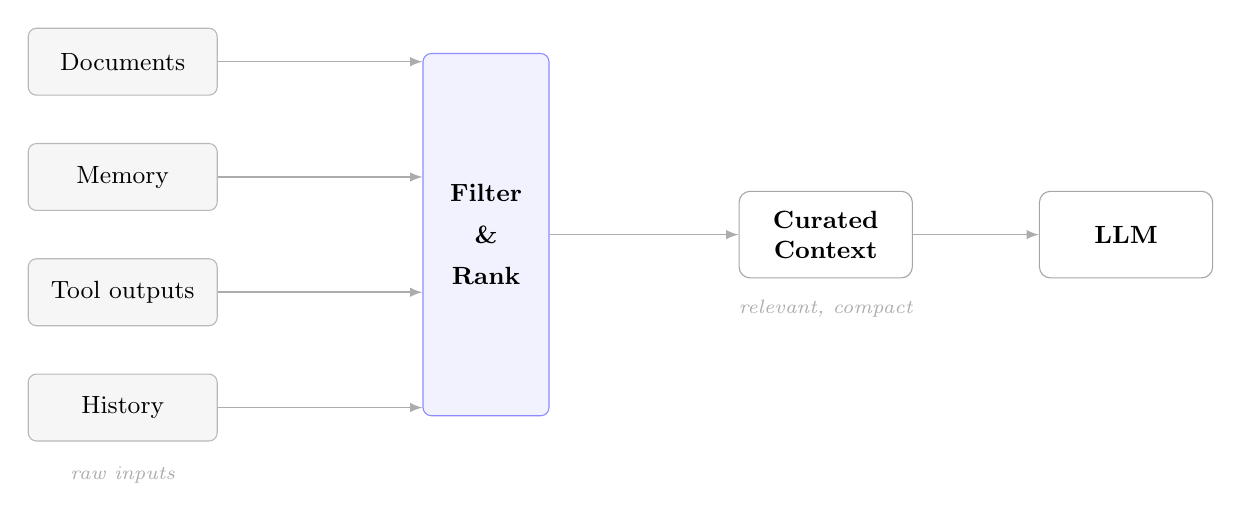
\begin{tikzpicture}[node distance=0.6cm and 2.6cm]

% --- 4 source nodes, vertical column ---
\node[srcbox]                 (docs)  {Documents};
\node[srcbox, below=of docs]  (mem)   {Memory};
\node[srcbox, below=of mem]   (tools) {Tool outputs};
\node[srcbox, below=of tools] (hist)  {History};
\node[annot,  below=2mm of hist] {raw inputs};

% --- Processor, vertically centred on the column ---
\node[procbox, right=of {$(docs.east)!0.5!(hist.east)$}] (proc)
    {Filter\\[4pt]\&\\[4pt]Rank};

% --- Output nodes ---
\node[outbox, right=2.4cm of proc] (ctx) {Curated\\Context};
\node[annot,  below=1.5mm of ctx]  {relevant, compact};
\node[outbox, right=1.6cm of ctx]  (llm) {LLM};

% --- Arrows: sources → proc (enter proc.west at matching heights) ---
\draw[arr] (docs.east)  -- (proc.west |- docs.east);
\draw[arr] (mem.east)   -- (proc.west |- mem.east);
\draw[arr] (tools.east) -- (proc.west |- tools.east);
\draw[arr] (hist.east)  -- (proc.west |- hist.east);

% --- Arrows: proc → outputs ---
\draw[arr] (proc.east) -- (ctx.west);
\draw[arr] (ctx.east)  -- (llm.west);

\end{tikzpicture}
\end{document}
